Apache Hadoop is an open-source framework for distributed storage of
large datasets and processing across clusters of computers. It was
created in 2006 after the release of GFS
\cite{Ghemawat:2003:GFS:1165389.945450} and MapReduce
\cite{Dean:2004:MSD:1251254.1251264} papers from Google. The core part
of Hadoop comprises of its distributed file system -- HDFS, and the
job scheduling, resource management framework -- YARN.

The attribute that makes the biggest difference in Hadoop and similar
projects is that of data locality awareness. In contrast to the HPC
architecture, we do not distinguish anymore between processing and
storage nodes. All nodes in a cluster perform both roles. Datasets are
split into blocks of data. To provide fault tolerance each block is
replicated in several nodes in the cluster. Moreover, there is a
central authority which keeps track of the nodes each block is stored.

With that feature in mind, we do not move datasets anymore to the
computing nodes but the executable of our job to the nodes where our
data reside. When the processing of the individual blocks is done, we
gather the result. That is a great paradigm shift from the traditional way
of processing big datasets. A high level overview of the Hadoop
architecture is depicted in Figure
\ref{fig:hadoop_arch_overview}. Datasets are split into blocks and
are stored in the nodes of cluster, both the original and the
replicas. When a user submits a job, the workflow manager will copy
the job to the appropriate nodes, which in parallel will execute
it. Finally, the workflow manager will gather the individual results,
aggregate them and return the final result to the client.

\begin{figure}
\centering
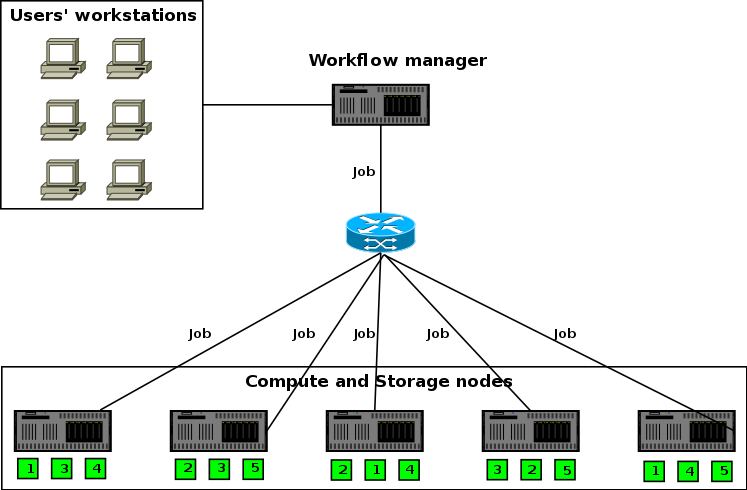
\includegraphics[scale=0.5]{resources/images/Background/hadoop_arch_overview.png}
\label{fig:hadoop_arch_overview}
\caption{Hadoop high level architecture}
\end{figure}